\documentclass{beamer}
\usepackage[resetfonts]{cmap}
\usepackage[T1]{fontenc}
\usepackage[utf8]{inputenc}
\usepackage[czech]{babel}
\usepackage{color}

\usetheme[compress]{Ilmenau}

\author[Martin Hořeňovský]{Martin Hořeňovský\\{\small Vedoucí práce: Michal Sojka}}
\title{Využití symbolické exekuce pro testování real-time bezpečnostně
kritického softwaru}
\institute{FEL ČVUT}
\date{2015}

\begin{document}
\begin{frame}
\titlepage
\end{frame}


\section{Úvod}
\subsection*{Symbolická exekuce}
\begin{frame}
\frametitle{Symbolická exekuce}
\begin{itemize}
    \item Umožňuje prozkoumat všechny průchody programem
    \item Nepotřebuje programátorem dodané vstupy
    \item Umožňuje najít chyby které se projeví až za běhu
    \item Extrémně náročná na výpočetní zdroje
    \item Některé konstrukce v kódu jsou neřešitelné
\end{itemize}
\begin{center}
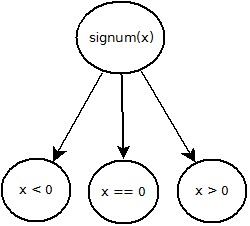
\includegraphics[scale=0.5]{symb-exec.png}
\end{center}
\end{frame}

\subsection*{KLEE}
\begin{frame}
\frametitle{KLEE}
\begin{itemize}
    \item KLEE vzniklo v roce 2008 jako nástroj pro automatické generování
    unit testů
    \item Umožňuje spustit podmnožinu jazyka C (vlákna, symbolické floaty, ASM nejsou podporovány)
    \item Pracuje na spustitelném programu převedeném do interní reprezentace LLVM nástrojů
\end{itemize}
\end{frame}

\begin{frame}
\begin{center}
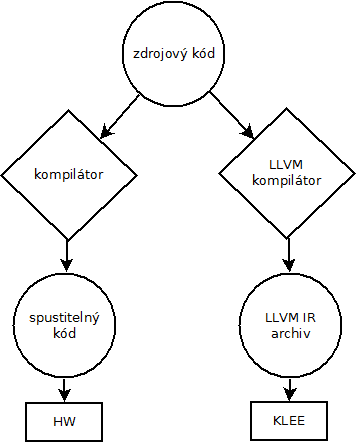
\includegraphics[scale=0.38]{kompilace.png}
\end{center}
\end{frame}

\subsection*{Cíl práce}
\begin{frame}
\frametitle{Cíl práce}
\begin{itemize}
    \item Prozkoumat možnost použití KLEE pro verifikaci bezpečnostně
    kritického, real-time softwaru
    \item Analýza eMotor softwaru pro řízení elektrických motorů
    \item Analýza MaCAN knihovny
    \item Návrh dalších vylepšení
    \vspace*{1cm}
    \item Dokumentace výsledků
\end{itemize}
\end{frame}

\subsection*{MaCAN}
\begin{frame}
\frametitle{MaCAN - Message Authenticated CAN}
\begin{itemize}
    \item CAN je standard pro industriální sítě
    \item Nemá v sobě žádné zabezpečení nebo autentifikaci
    \item MaCAN je zpětně kompatibilní nadstavba na CANu, umožňující
    podepisovat zprávy
    \item Knihovna implementovaná katedrou řídící techniky
\end{itemize}
\end{frame}

\section{Práce}
\subsection*{Modifikace MaCAN knihovny}
\begin{frame}
\frametitle{Modifikace MaCAN knihovny}
\begin{itemize}
    \item MaCAN knihovna má silně abstrahované HW závislosti
    \begin{itemize}
    \item Většina práce tedy spočívala v doplnění KLEE "hardwaru"
    \end{itemize}
    \item Byl vytvořen klient pro práci s knihovnou
    \item Vzhledem ke svému účelu používá kryptografická primitiva, která bylo
    potřeba obejít
\end{itemize}
\end{frame}


\section{Výsledky}
\subsection*{Nalezitelné chyby}
\begin{frame}
\frametitle{Nalezitelné chyby}
\begin{itemize}
    \item Assertion violation
    \item Přístup k nealokované paměť
    \item Dělení nulou
    \item Přetečení integrální aritmetiky
\end{itemize}
\end{frame}

\subsection*{Nalezené chyby}
\begin{frame}
\frametitle{Nalezené chyby}
\begin{itemize}
    \item Testování nalezlo 10 potenciálních problémů, všechny v integrální aritmetice
    \item 3 z nich byly reálné chyby
    \item 1 byla nalezena jíž dříve
    \item 1 byla opravena
    \item 1 je neškodná pro současné implementace HW závislostí
\end{itemize}
\end{frame}

\subsection*{Evaluace}
\begin{frame}
\frametitle{Evaluace}
\begin{itemize}
    \item MaCAN knihovna v testované konfiguraci má 1340 LOC, 1700 instrukcí
    \item Nejlepší běh pokryl 60\% všech větví a 77\% všech instrukcí
    \item Výsledky jsou z běhu dlouhého 5 dní
    \item Celkové výsledky byly dostatečně dobré, aby bylo KLEE přidáno mezi
    způsoby testování MaCAN knihovny
\end{itemize}
\end{frame}

\subsection*{Problémy}
\begin{frame}
\frametitle{Problémy}
\begin{itemize}
    \item Miskonfigurace verifikovaného programu může vést k nalezení neexistujících chyb
    \item Defaultní heuristika vede k zaseknutí KLEE (chyba v paměťové alokaci)
    \item Ani při 100\% pokrytí by analýza nebyla kompletní
    \begin{itemize}
        \item Musel jsme obejít kryptografii
        \item Netestoval jsem všechny možné konfigurace knihovny
    \end{itemize}
\end{itemize}
\end{frame}


\section{Závěr}
\subsection*{Možná pokračování}
\begin{frame}
\frametitle{Možné pokračování}
\begin{enumerate}
    \item Heuristika pro prioritní pokrytí chybových stavů
    \item Přidání detekcí dalších chyb
    \item Možnost označit specifickou chybu za neškodnou
\end{enumerate}
\end{frame}

\subsection*{KONEC}
\begin{frame}
\begin{center}
{\bf\Large Děkuji za pozornost}
\end{center}
\end{frame}

\appendix
\section{Poznámky k posudku}
\subsection{Problémy}
\begin{frame}
\frametitle{Více problémů nalezeno přes dfs10}
    Jedná se o přehlédnutí v tabulce, dfs10 má větší pokrytí.
    \begin{center}
    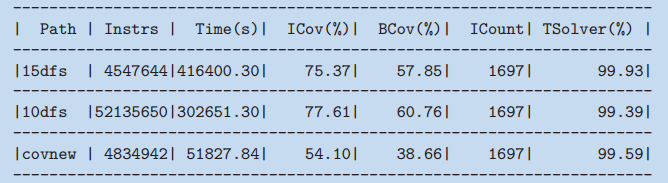
\includegraphics[scale=0.6]{tabulka.png}
    \end{center}
\end{frame}

\begin{frame}
\frametitle{Ostatní}
\begin{enumerate}
    \item Hloubka zpráv
    \begin{itemize}
        \item covnew spuštění běžel s hloubkou 15 stránek.
    \end{itemize}
    \item Doba běhu
    \begin{itemize}
        \item Měření není přesné, dochází k dilataci (extrémní případ je zaseklý covnew)
        \item Tabulka 4.7 používá data z nejúspěšnějšího běhu, který běžel kratší dobu
    \end{itemize}
    \item Paměťové nároky a pokrytí se s časem zvětšují
\end{enumerate}
\end{frame}

\end{document}
